%
% fft.tex -- Fast Fourier Transform
%
% (c) 2018 Prof Dr Andreas Müller, Hochschule Rapperswil
%
\subsubsection{Fast Fourier Transform}
\index{Fast Fourier Transform}
Die komplexe Darstellung der diskreten Fourier-Transformation ermöglicht
eine Formulierung, in der die Berechnung der Koeffizienten wie auch die
Auswertung des trigonometrischen Polynoms sehr viel schneller erfolgen
kann, wenigstens wenn $N$ gerade ist.
Die Bestimmung der $c_l$ verlangt die Berechnung der Produkte
$y_j e^{lt_j}$ für alle $j$ und $l$.
Ausserdem ist $t_j=2\pi j/N=lt_1$, die Exponentialfaktoren sind daher
$e^{lt_j}=(e^{t_1})^{lj}$.
Die Details dieses Algorithmus sollen hier nicht entwickelt werden,
es soll nur der Rechenaufwand abgeschätzt werden.
Die Anzahl der Multiplikationen dominiert die Laufzeit der Berechnung,
daher soll $g(N)$ die Anzahl der Multiplikationen für eine
Fourier-Transformation mit $N$ Termen bezeichnen.

Da $N$ gerade ist, kann man die Summe zur Berechnung der Koeffizienten
\begin{align}
c_l
&=
\sum_{j=0}^{N-1} y_j e^{-ilt_j}
\intertext{aufteilen in gerade und ungerade Terme}
&=
\sum_{j=0}^{N/2-1} y_{2j} e^{-ilt_{2j}}
+
\sum_{j=0}^{N/2-1} y_{2j+1} e^{-ilt_{2j+1}}
\notag
\\
&=
\sum_{j=0}^{N/2-1} y_{2j} e^{-ilj t_{2}}
+
e^{-ilt_1}
\sum_{j=0}^{N/2-1} y_{2j+1} e^{-ilj t_{2}}.
\label{skript:fft:split}
\end{align}
Es ist zu erkennen, dass jeder Summand eine Fourier-Transformation
mit der halben Anzahl von Datenpunkten und der doppelten Schrittweite
$t_2$ statt $t_1$ ist.
Schreiben wir 
\[
\begin{aligned}
y'_j
&= 
y_{2j}&j&=0,\dots,\frac{N}2
\\
y''_j
&=
y_{2j+1}&j&=0,\dots,\frac{N}2
\end{aligned}
\]
für die geraden bzw.~ungeraden Elemente, dann ist er erste Summand in
\eqref{skript:fft:split} die Fouriertransformation von $y'$, der zweite
Summand enthält die Fouriertransformation von $y''$, es ist also
\[
c_l = c'_l + e^{-ilt_1} c''_l.
\]
Der zusätzliche Aufwand für die Berechnung von $c_l$ aus $c'_l$ und $c''_l$
ist also nur gerade eine Multiplikation mit einem Exponentialfaktor.

Der Aufwand für die Berechnung der Koeffizienten $c_l$ setzt sich also
zusammen aus dem Aufwand für zwei Fourier-Transformationen mit Länge $N/2$
und $N$ Multiplikationen, eine für jeden der Koeffizienten $c_l$.
Dies führt auf die Rekursionsformel
\begin{equation}
g(N) = 2g(N/2) + N.
\label{skript:fft:rekursion}
\end{equation}
Wenn $N=2^m$ sogar eine Zweierpotenz ist, dann lässt sich diese
Idee iterieren und damit $g(2^m)$ iterativ aus $g(2)$ berechnen.

Die Rekursionsformel
\eqref{skript:fft:rekursion}
hat die Lösung $g(N) = N\log_2 N$, wie man durch Einsetzen in die
rechte Seite von
\eqref{skript:fft:rekursion}
prüfen kann:
\[
2g(N/2) + N
=
2\cdot\frac{N}2\log_2\frac{N}2 + N
=
N(\log_2 N - 1) + N
=
N\log_2 N
=
g(N).
\]
Wir schliessen daraus, dass der Aufwand für die Berechnung der
Fourier-Transformation mit diesem Algorithmus von der Grössenordnung
$O(N\log N)$ ist, also deutlich schneller als die naive Berechnung
mit der Summenformel, die Aufwand $O(N^2)$ verlangt.
\begin{figure}
\centering
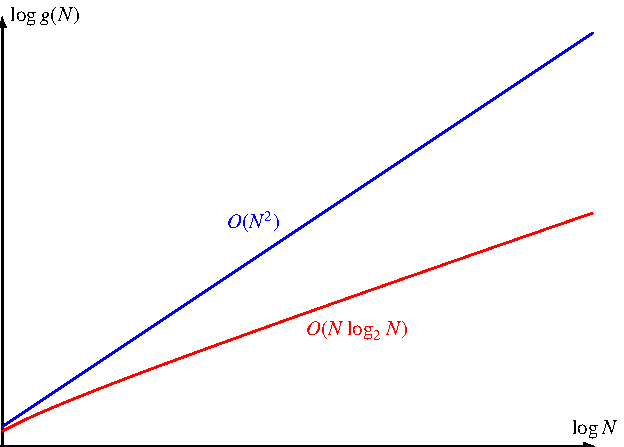
\includegraphics{chapters/6/fftaufwand.pdf}
\caption{Aufwand für die komplexe Fouriertransformation ({\color{blue}blau})
im Vergleich mit
dem Aufwand für die schnelle Fourier-Transformation ({\color{red}rot}).
\label{skript:fft:aufwandgraph}}
\end{figure}
In Abbildung~\ref{skript:fft:aufwandgraph} sind die beiden Aufandkurven im 
Vergleich dargestellt.

Diese schnelle Variante der Fourier-Transformation wurde von Cooley 
\index{Cooley, J.~W.}%
und Tukey 1965 veröffentlicht.
\index{Tukey, J.~T.}%
Das Verfahren war allerdings auch schon Carl Friedrich Gauss bekannt,
\index{Gauss, Carl Friedrich}
er hat es zur Berechnung der Bahnelemente der Asteroiden Pallas und
Juno verwendet.
Der Algorithmus wird von vielen Softwarepaketen für numerische Berechnung
implementiert.
Sehr verbreitet ist die Bibliothek FFTW3 (Fastest Fourier Transform in the
West, Version 3) \cite{skript:fftw}. 
Diese Bibliothek wird zum Beispiel auch von Octave verwendet um die
Funktion \texttt{fft} zu implementieren.
\index{fft@\texttt{fft}}%
Sie ist sehr einfach zu verwenden: als Argument wird der Vektor der
$y$-Werte übergeben, der Rückgabewert ist der Vektor der komplexen
Koeffizienten $c_l$.
Der Koeffizient $c_0$ ist das erste Element im Rückgabevektor, gefolgt
von $c_1,\dots,c_{N/2-1}$.
Der Koeffizient $c_{-1}$ ist das letzte Element im Rückgabevektor, davor
steht $c_{-2}$.
Als Zeilenvektor geschrieben ist der Rückgabewert von \texttt{fft}
\[
( c_0, c_1, c_2, \dots , c_{n-1}, c_n=c_{-n},
c_{-n+1},c_{-n+2},\dots, c_{-2},c_{-1}).
\]


%Für reelle Werte $y_j$ haben die Koeffizienten $c_l$ zusätzliche
%Symmetrieeigenschaften.
%Die komplex konjugierte $\bar c_l$ ist
%\[
%\bar c_l
%=
%\overline{\sum_{j=0}^{N-1} y_j e^{2\pi ijl/N}}
%=
%\sum_{j=0}^{N-1} y_j e^{-2\pi i jl/N}
%=
%c_{-l}.
%\]
%Daraus liest man zum Beispiel ab, dass $c_0\in\mathbb R$ ist, nämlich
%\[
%c_0 = \frac{1}{N} \sum_{j=0}^{N-1} y_j = a_0.
%\]
%Für die anderen Koeffizienten gilt zunächst
%\begin{align*}
%c_l
%&=
%\frac{1}{N}\sum_{j=0}^{N-1} y_j e^{-2\pi ilj/N}
%=
%\frac{1}{N}\sum_{j=0}^{N-1} y_j \biggl(\cos \frac{2\pi lj}{N} + i \sin\frac{2\pi lj}{N}\biggr)
%\\
%&=
%\frac{1}{N}\sum_{j=0}^{N-1} y_j
%\cos \frac{2\pi lj}{N}
%+
%i
%\frac{1}{N}\sum_{j=0}^{N-1} y_j
%\sin\frac{2\pi lj}{N}
%\\
%&=
%\frac12(a_l + ib_l)
%\end{align*}
%Zusammen mit der Beziehung $\bar c_l=c_{-l}$, können wir die reellen
%Fourier-Koeffizienten auch verwenden, um die reellen Koeffizienten
%\begin{align*}
%a_l
%&=
%c_l + c_{-l}
%&&\text{und}&
%b_l
%&=
%\frac1{i}
%(c_l - c_{-l})
%\end{align*}
%durch die komplexen Koeffizienten auszudrücken.

In der Übungsaufgabe zu diesem Kapitel wird verlangt die
Fourier-Koeffizienten von Hand zu berechnen.
Mit der Funktion \texttt{fft} in Octave kann dies jetzt natürlich viel
schneller erreicht werden.
Wendet man \texttt{fft} auf den Vektor
\[
y = (-3.2, -13.6, -12.3, -3.9, 3.1, 2.0, -4.1, -6.1, 0.5, 10.7, 16.3, 10.6 )
\]
erhält man einen Vektor mit 12 komplexen Fourier-Koeffizienten.
Wie im letzten Abschnitt erklart, können wir die reellen Fourier-Koeffizienten
$a_k$ und $b_k$ wieder erkennen.
Man liest ab:
\[
\texttt{fft}(y) / 6
=
\left[
\begin{tabular}{>{\tt}r}
   0.00000 + 0.00000i\\
   0.34210 + 7.52778i\\
  -3.57500 + 9.16544i\\
   0.08333 + 0.25000i\\
  -0.12500 + 0.15877i\\
   0.02456 + 0.02222i\\
   0.10000 + 0.00000i\\
   0.02456 - 0.02222i\\
  -0.12500 - 0.15877i\\
   0.08333 - 0.25000i\\
  -3.57500 - 9.16544i\\
   0.34210 - 7.52778i
\end{tabular}
\right]
\qquad\Rightarrow\qquad
\begin{tabular}{|>{$}c<{$}|>{$}r<{$}|>{$}r<{$}|}
\hline
k     &\hat{a}_k&\hat{b}_k\\
\hline
0     & 0.00000&        \\
1     & 0.34210&-7.52778\\
2     &-3.57500&-9.16544\\
3     & 0.08333&-0.25000\\
4     &-0.12500&-0.15877\\
5     & 0.02456&-0.02222\\
6     & 0.10000&        \\
\hline
\end{tabular}
\]
Die direkte Berechnung in der Aufgabe~1 führt auf die gleichen Werte.



